\section{Introduction}
\label{sec:intro}
 The Center of Aeronautical Studies (CEA) of the Federal University of Minas Gerais (UFMG) in Brazil was founded in 1964 with the aspiration to be a place where the students of Aeronautical Engineering could put in practice what they learn in class. The center was responsible for the design, construction and testing of more than ten flight proven airplanes throughout its history. It started by designing a glider for training, named Gaivota, seagull in Portuguese, then designing a high performance glider, transitioned to propelled aircraft during the eighties and now has its attention drawn specially to racer aircraft. The two newest designs, CEA308 and CEA311 (dubbed Anequim, the Portuguese name for the Mako shark), have the world record for the faster airplane under 300kg and 500kg of take-off wight, respectively. Now, CEA's newest endeavour in developing an all electrical racer airplane (\cref{fig:blueprint}). 
 
 \begin{figure}
     \centering
     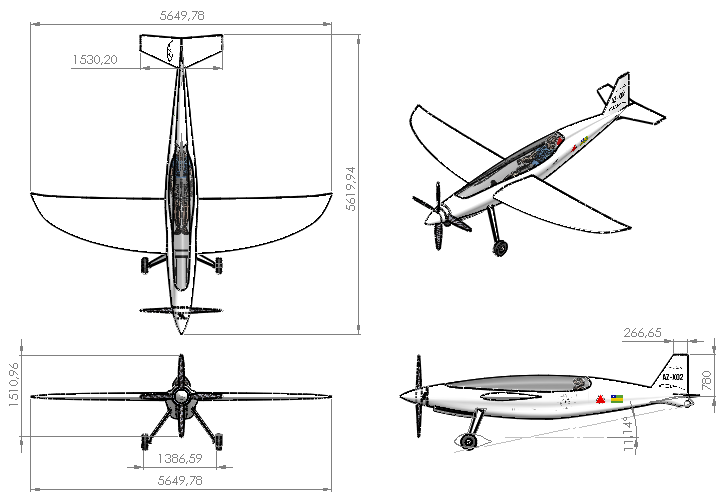
\includegraphics[width=\textwidth]{fig/AZX02_AP.png}
     \caption{Blueprint of CEA's new electric racer airplane. Courtesy of Danilo Azevedo (\url{dcrazevedo@gmail.com}).}
     \label{fig:blueprint}
 \end{figure}
 
 Electric propulsion presents a different challenge from conventional propulsion. 
 Although modern electrical engines can be lighter and smaller than conventional ones for the same power output,
  energy storage with batteries is much more complicated than simply storing fuel. This paper attempts to solve one particular problem of energy storage in batteries for aeronautical: removing heat generated by the batteries. Unlike aviation fuel, batteries do heat up when discharging and this heat must be dissipated to avoid damaging the batteries, which have a strict operating temperature window.

In this paper, three different solutions for battery cooling are analyzed. 
Firstly, the simplest, cheapest and lightest solution possible: no cooling at all.
The heat from the battery is simply conducted out of the airframe by the fuselage itself. 
The drawback of this solution is very low capacity of heat extraction.
The second proposed solution is to remove heat by forced convection with outside air channeled via a NACA inlet or a ram inlet. 
This allows for much higher cooling rates with not much weight added. 
The NACA inlet also has the advantage of increasing drag only slightly.


%Outline (escrever descricao de cada secao)
This paper is organized as follows. 
\Cref{sec:methods} deals with the physical modelling of the two competing solutions. 
\Cref{sec:results} presents the preliminary design of each solution, that is,
    batteries operating temperature, and
    the drag and weight penalties incurred if a particular solution is chosen.
\Cref{sec:discussion} presents a in depth analysis of the results obtained 
and attempts to choose the best compromise, and
\cref{sec:conclusion} concludes this work.
